\documentclass[handout]{beamer}  

%Smaller gap at between top and bottom of block when there are displayed equations
\addtobeamertemplate{block begin}{\setlength\abovedisplayskip{0pt}}
{\setlength{\belowdisplayskip}{0pt}}


\usepackage{setspace}
\linespread{1.3}
\usepackage{amssymb, amsmath, amsthm} 
\usepackage{rotating}
\usepackage{multirow}
\usepackage{graphicx}
\usepackage{synttree}
\usepackage{verbatim}
\usepackage{fancybox}
\usepackage{color}
\usepackage{tikz}
\usetikzlibrary{shapes,backgrounds}
\usepackage{hyperref}
\usetikzlibrary{trees}
\newcommand{\p}{\mathbb{P}}
\newcommand{\expect}{\mathbb{E}}
\newcommand{\var}{\mathbb{V}}



%\setbeamertemplate{blocks}[rounded][shadow=true] 
%gets rid of bottom navigation bars
\setbeamertemplate{footline}{
   \begin{beamercolorbox}[ht=4ex,leftskip=0.3cm,rightskip=0.3cm]{author in head/foot}
%    \usebeamercolor{UniBlue}
    \vspace{0.1cm}
    %\insertshorttitle \ - \insertdate 
    \hfill \insertframenumber / \inserttotalframenumber
   \end{beamercolorbox}
   \vspace*{0.1cm}
} 

%gets rid of navigation symbols
\setbeamertemplate{navigation symbols}{}


%Include or exclude the notes?
%\setbeameroption{show notes}
\setbeameroption{hide notes}


\title[Econ 103]{Economics 103, Statistics for Economists} 
\author[F. DiTraglia]{Francis J.\ DiTraglia}
\institute{University of Pennsylvania}
\date{Lecture 16}


\begin{document} 




%%%%%%%%%%%%%%%%%%%%%%%%%%%%%%%%%%%%%%%%

\begin{frame}[plain]
	\titlepage 
	

\end{frame} 


%%%%%%%%%%%%%%%%%%%%%%%%%%%%%%%%%%%%%%%%


\begin{frame}

\centering \Huge Confidence Intervals -- Part I

\end{frame}
%%%%%%%%%%%%%%%%%%%%%%%%%%%%%%%%%%%%%%%%

\begin{frame}
\frametitle{What We've Done So Far}

\begin{itemize}
\item Random Sampling: $X_1, \hdots, X_n \sim \mbox{ iid}$ 
\item Use estimator $\widehat{\theta}$ to learn about population parameter $\theta_0$ 
\item Estimator $\widehat{\theta}$ is a random variable: 
	\begin{itemize}
		\item Distribution of $\widehat{\theta}$ is called \emph{sampling distribution}
		\item Bias of an estimator 
		\item Variance of an estimator 
		\item Mean-squared Error (MSE) of an estimator 
		\item Consistency of an Estimator
	\end{itemize}
\end{itemize}


\end{frame}
%%%%%%%%%%%%%%%%%%%%%%%%%%%%%%%%%%%%%%%%

\begin{frame}
\frametitle{Inference}

\begin{block}{Confidence Intervals}
What values of $\theta_0$ are consistent with the data we observed?
\end{block}

\begin{block}{Hypothesis Testing}
I think that $\theta_0 = 0$. Do the data we observed suggest that I should change my mind?
\end{block}


\end{frame}
%%%%%%%%%%%%%%%%%%%%%%%%%%%%%%%%%%%%%%%%
\begin{frame}
\frametitle{Am I Taller Than The Average American Male? \hfill 
\includegraphics[scale = 0.05]{./images/clicker}}

\framesubtitle{\href{http://www.cdc.gov/nchs/data/series/sr_11/sr11_252.pdf}{\fbox{Source: Centers for Disease Control (pg.\ 16)}}}

My height is 73 inches. Based on a sample of US males aged 20 and over, the Centers for Disease Control (CDC) reported a mean height of about 69 inches in a recent report.

\vspace{2em}



\alert{Clearly I'm taller than the average American male!}\\
Do you agree or disagree?
\begin{enumerate}[(a)]
	\item Agree
	\item Disagree
	\item Not Sure
\end{enumerate}
\end{frame}
%%%%%%%%%%%%%%%%%%%%%%%%%%%%%%%%%%%%%%%%
\begin{frame}
\frametitle{Remember: The Sample Mean is Random!}

\alert{Just because the sample mean is 69 inches it doesn't follow that the population mean is 69 inches!}


\begin{block}{What Else Should We Consider?}
	\begin{itemize}\pause
		\item How big was the sample? \pause
			\begin{itemize}
				\item If the sample was very small there's a higher chance that it won't be representative of the population as a whole \pause
				\item Why? The variance of the sample mean is \emph{decreasing with sample size} so bigger samples are less noisy. \pause
			\end{itemize}
		\item How much variability is there in height in the population?	\pause
			\begin{itemize}
				\item If everyone is very similar in height, any sample we take will be representative of the population. \pause
				\item Remember: the variance of the sample mean is \emph{increasing} with the population standard deviation. 
			\end{itemize}
	\end{itemize}
\end{block}

\end{frame}
%%%%%%%%%%%%%%%%%%%%%%%%%%%%%%%%%%%%%%%%
\begin{frame}
\frametitle{Am I Taller Than The Average American Male?}
\framesubtitle{\href{http://www.cdc.gov/nchs/data/series/sr_11/sr11_252.pdf}{\fbox{Source: Centers for Disease Control (pg.\ 16)}}}

	
	\begin{table}[h]
	\caption{Height in inches for Males aged 20 and over (approximate)}
		\begin{tabular}{|lr|}
		\hline
			Sample Mean & 69 inches\\
			Sample Std.\ Dev.\ & 6 inches\\
			Sample Size & 5647 \\
			\hline
			My Height & 73 inches\\
			\hline
		\end{tabular}
	\end{table}

\vspace{2em}
\alert{We'll return to this example later.}

\end{frame}
%%%%%%%%%%%%%%%%%%%%%%%%%%%%%%%%%%%%%%%%

\begin{frame}
\frametitle{For Now -- Single Population, Normally Distributed}
\Large
$$\boxed{X_1, X_2, \hdots, X_n\sim \mbox{iid } N(\mu,\sigma^2)}$$


\vspace{4em}
\normalsize
\alert{Later we'll look at more than one population and talk about what happens if Normality doesn't hold.}
\end{frame}
%%%%%%%%%%%%%%%%%%%%%%%%%%%%%%%%%%%%%%%%

\begin{frame}
\frametitle{
\includegraphics[scale = 0.05]{./images/clicker}}
Suppose $X_1, X_2, \hdots, X_n \sim \mbox{iid } N(\mu,\sigma^2)$. What is the sampling distribution of $\sqrt{n}(\bar{X}_n - \mu)/\sigma$?


\begin{enumerate}[(a)]
\item $N(\mu, \sigma^2)$
\item $N(0,1)$
\item $N(0,\sigma)$
\item $N(\mu, 1)$
\item Not enough information to determine.
\end{enumerate}

\end{frame}

%%%%%%%%%%%%%%%%%%%%%%%%%%%%%%%%%%%%%%%%
\begin{frame}
\frametitle{Z-score!}
Suppose $X_1, X_2, \hdots, X_n \sim \mbox{iid } N(\mu,\sigma^2)$. From above,
	\begin{eqnarray*}
			E[\bar{X}_n] &=& \mu\\
			Var(\bar{X}_n) &=&  \sigma^2/n\\ 
			&\Rightarrow& SD(\bar{X}_n) =\sigma/\sqrt{n}
	\end{eqnarray*} 
Thus,
	$$\sqrt{n}(\bar{X}_n - \mu)/\sigma =  \frac{\bar{X}_n - \mu}{\sigma/\sqrt{n}} =  \frac{\bar{X}_n - E[\bar{X}_n]}{SD(\bar{X}_n)}  \sim N(0,1)$$
Remember that we call the standard deviation of a sampling distribution the \alert{standard error}, written $SE$, so $$\frac{\bar{X}_n - \mu}{SE(\bar{X}_n)} \sim N(0,1)$$
\end{frame}
%%%%%%%%%%%%%%%%%%%%%%%%%%%%%%%%%%%%%%%%

\begin{frame}
\frametitle{
\includegraphics[scale = 0.05]{./images/clicker}}
Suppose $X_1, X_2, \hdots, X_n \sim \mbox{iid } N(\mu,\sigma^2)$. What is the approximate value of the following?
	$$\p\left(-2 \leq \frac{\bar{X}_n - \mu}{SE(\bar{X}_n)} \leq 2 \right)\pause \alert{\approx 0.95}$$

\end{frame}

%%%%%%%%%%%%%%%%%%%%%%%%%%%%%%%%%%%%%%%%
\begin{frame}
\frametitle{What happens if I rearrange?}
	\begin{eqnarray*}
		P\left(-2 \leq \frac{\bar{X}_n - \mu}{SE(\bar{X}_n)} \leq 2 \right) &=& 0.95\\ \\ \pause
			P\left(-2\cdot SE\leq \bar{X}_n - \mu \leq 2 \cdot SE\right) &=& 0.95\\ \\ \pause
			P\left(-2\cdot SE - \bar{X}_n \leq - \mu \leq 2 \cdot SE - \bar{X}_n \right) &=& 0.95\\ \\ \pause
			\alert{P\left( \bar{X}_n - 2\cdot SE \leq \mu \leq \bar{X}_n + 2\cdot SE \right)}&\alert{=}& \alert{0.95}
	\end{eqnarray*}

\end{frame}

%%%%%%%%%%%%%%%%%%%%%%%%%%%%%%%%%%%%%%%%

% \begin{frame}
% \frametitle{What Happens if I Rearrange?}
% \begin{eqnarray*}
% X_1, X_2, \hdots, X_n\sim \mbox{iid } N(\mu,\sigma^2) &\Rightarrow& \bar{X}_n \sim N(\mu, \sigma^2/n)\\ \pause
% 	&\Rightarrow& \alert{\frac{\bar{X}_n - \mu}{\sigma/\sqrt{n}} \sim N(0,1)}
% \end{eqnarray*}
% \pause
% \begin{eqnarray*}
% 	 P\left(  -2\leq\frac{\bar{X}_n - \mu}{\sigma/\sqrt{n}} \leq 2\right) &=& 0.95\\ \pause
% 	P\left( - 2 \frac{\sigma}{\sqrt{n}}\leq \bar{X}_n - \mu \leq 2 \frac{\sigma}{\sqrt{n}}\right)&=&0.95\\ \pause
% 		P\left(- 2 \frac{\sigma}{\sqrt{n}} - \bar{X}_n \leq - \mu \leq 2 \frac{\sigma}{\sqrt{n}} - \bar{X}_n\right)&=&0.95\\ \pause
% P\left( \bar{X}_n - 2 \frac{\sigma}{\sqrt{n}}\leq \mu \leq \bar{X}_n + 2 \frac{\sigma}{\sqrt{n}}\right)&=&0.95
% \end{eqnarray*}
% \end{frame}

% %%%%%%%%%%%%%%%%%%%%%%%%%%%%%%%%%%%%%%%%
\begin{frame}
\frametitle{Confidence Intervals}

\begin{block}{Confidence Interval (CI)}
A confidence interval is a range $(A,B)$ constructed from the \alert{sample data} that has a specified probability of containing a \alert{population parameter}:
	$$P(A \leq \theta_0 \leq B) = 1-\alpha$$
\end{block} 

\pause

\begin{block}{Confidence Level}
The \alert{specified probability}, typically denoted $1-\alpha$, is called the confidence level. For example, if $\alpha = 0.05$ then the confidence level is 0.95 or 95\%.
\end{block}
\end{frame}
%%%%%%%%%%%%%%%%%%%%%%%%%%%%%%%%%%%%%%%%

\begin{frame}
\frametitle{Confidence Interval for Mean of Normal Population}
\framesubtitle{Population Variance Known}


\begin{block}{Confidence Interval for Mean of Normal Population}
	The interval \alert{$\boxed{\bar{X}_n \pm 2 \sigma/\sqrt{n}}$} has approximately 95\% probability of containing the population mean $\mu$, provided that:
		$$\boxed{X_1, X_2, \hdots, X_n\sim \mbox{iid } N(\mu,\sigma^2)}$$
\end{block}

\pause

\begin{alertblock}{But What Does This Mean?}
\end{alertblock}

\end{frame}
%%%%%%%%%%%%%%%%%%%%%%%%%%%%%%%%%%%%%%%%

\begin{frame}
\frametitle{Which quantities are random?\hfill 
\includegraphics[scale = 0.05]{./images/clicker}}
Suppose $X_1, X_2, \hdots, X_n\sim \mbox{iid } N(\mu,\sigma^2)$.
Which quantities are random variables?
	\begin{enumerate}[(a)]
\item $\mu$ only
\item $\sigma$ and $\mu$
\item $\sigma$ only
\item $\sigma, \mu$ and $\bar{X}_n$
\item $\bar{X}_n$ only
\end{enumerate}

\vspace{1em}
\pause
\alert{\large $\bar{X}_n$ only.}

\end{frame}
%%%%%%%%%%%%%%%%%%%%%%%%%%%%%%%%%%%%%%%%
\begin{frame}
\frametitle{Confidence Interval is a Random Variable!}
\begin{enumerate}
	\item $X_1, \hdots, X_n$ are RVs $\Rightarrow \bar{X}_n$ is a RV (repeated sampling) \pause
	\item $\mu$, $\sigma$ and $n$ are constants \pause
	\item Confidence Interval $\bar{X_n}\pm 2 \sigma/\sqrt{n}$ is also a RV!
\end{enumerate}


\end{frame}

%%%%%%%%%%%%%%%%%%%%%%%%%%%%%%%%%%%%%%%
\begin{frame}
\frametitle{Meaning of Confidence Interval}
\begin{block}{Meaning of Confidence Interval}
If we sampled many times we'd get many different sample means, each leading to a \alert{different} confidence interval. Approximately 95\% of these intervals will contain $\mu$.
\end{block}
 

\begin{block}{Rough Intuition}
What values of $\mu$ are consistent with the data?
\end{block}

\end{frame}




\begin{frame}
\frametitle{CI for Population Mean: Repeated Sampling}

\begin{center}
\setlength{\unitlength}{1cm}
\begin{picture}(5,7)
\put(-0.5,6){\framebox(6,1){$X_1, X_2, \hdots, X_n \sim \mbox{iid } N(\mu, \sigma^2)$}}

\pause

\put(0.5,6){\vector(-1,-1){1.5}}
\put(-2.3,3.7){\framebox(2.5,0.65){Sample 1}}

\pause

\put(-1,3.5){\vector(0,-1){0.75}}
\put(-1.25,2.1){\framebox(0.5,0.5){\small $\bar{x}_1$}}

\pause

\put(-1,2){\vector(0,-1){0.5}}
\put(-1.7,1){{\small $\bar{x}_1 \pm 2\sigma/\sqrt{n}$}}

\pause

\put(2,6){\vector(0,-1){1.5}}
\put(0.7,3.7){\framebox(2.5,0.65){Sample 2}}

\pause

\put(2,3.5){\vector(0,-1){0.75}}
\put(1.75,2.1){\framebox(0.5,0.5){\small $\bar{x}_2$}}

\pause

\put(2,2){\vector(0,-1){0.5}}
\put(1.35,1){{\small $\bar{x}_2 \pm 2\sigma/\sqrt{n}$}}

\pause

\put(3.8,4){\makebox{...}}
\put(3.8,2.3){\makebox{...}}

\pause

\put(4.5,6){\vector(1,-1){1.5}}
\put(4.8,3.7){\framebox(2.5,0.65){Sample M}}

\pause

\put(6,3.5){\vector(0,-1){0.75}}
\put(5.75,2.1){\framebox(0.5,0.5){\small $\bar{x}_M$}}

\pause

\put(6,2){\vector(0,-1){0.5}}
\put(5.35,1){{\small $\bar{x}_M \pm 2\sigma/\sqrt{n}$}}

\pause

\put(-1,0.2){\makebox{\small Repeat $M$ times $\rightarrow$  get $M$ different intervals}}

\pause

\put(-1,-0.3){\makebox{\small \alert{Large M $\Rightarrow$ Approx.\ 95\% of these Intervals Contain $\mu$}}}

\end{picture}
\end{center}


\end{frame}
%%%%%%%%%%%%%%%%%%%%%%%%%%%%%%%%%%%%%%%%
\begin{frame}
\frametitle{Simulation Example: $X_1, \hdots, X_5 \sim \mbox{iid } N(0,1)$, $M = 20$}

\begin{figure}
\centering
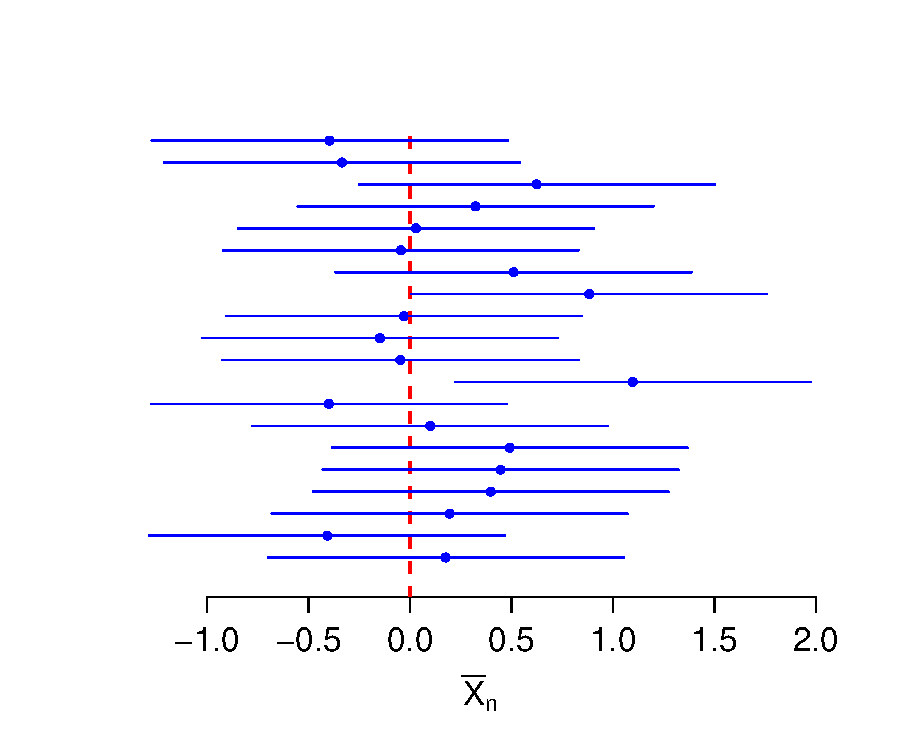
\includegraphics[scale = 0.5]{./images/CIs1}
\caption{Twenty confidence intervals of the form $\bar{X}_n \pm 2 \sigma/\sqrt{n}$ where $n=5$, $\sigma^2 = 1$ and the true population mean is $0$.}
\end{figure}

\end{frame}

%%%%%%%%%%%%%%%%%%%%%%%%%%%%%%%%%%%%%%%%
\begin{frame}
\frametitle{Meaning of Confidence Interval for $\theta_0$}
	$$\boxed{P(A\leq \theta_0 \leq B) = 1-\alpha}$$
Each time we sample we'll get a different confidence interval, corresponding to different realizations of the random variables $A$ and $B$. If we sample many times, approximately $100\times(1-\alpha)$\% of these intervals will contain the population parameter $\theta_0$.

\end{frame}





%%%%%%%%%%%%%%%%%%%%%%%%%%%%%%%%%%%%%%%%
\begin{frame}
\frametitle{True or False? \hfill 
\includegraphics[scale = 0.05]{./images/clicker}}
Suppose 
	$$\boxed{X_1, X_2, \hdots, X_n\sim \mbox{iid } N(\mu,\sigma^2)}$$
Then, there is about about a 95\% chance that the population mean $\mu$ lies in the interval $\bar{X}_n \pm 2 \sigma/\sqrt{n}$.

\vspace{1em}

\begin{enumerate}[(a)]
\item True
\item False
\end{enumerate}


\pause
\vspace{1em}
\alert{\huge FALSE! -- $\mu$  is a constant!}


\end{frame}
%%%%%%%%%%%%%%%%%%%%%%%%%%%%%%%%%%%%%%%%
\begin{frame}
\frametitle{Confidence Intervals: Some Terminology}
\begin{block}{Margin of Error}
When a CI takes the form $\widehat{\theta}\pm ME$, $ME$ is the Margin of Error. 
\end{block}
\pause
\begin{block}{Lower and Upper Confidence Limits}
The lower endpoint of a CI is the \alert{lower confidence limit (LCL)}, while the upper endpoint is the \alert{upper confidence limit (UCL)}.
\end{block}
\pause
\begin{block}{Width of a Confidence Interval}
The distance $\alert{|\mbox{UCL} - \mbox{LCL}|}$ is called the \alert{width} of a CI. This means exactly what it says. 
\end{block}

\end{frame}
%%%%%%%%%%%%%%%%%%%%%%%%%%%%%%%%%%%%%%%%
\begin{frame}
\frametitle{What is the Margin of Error\hfill 
\includegraphics[scale = 0.05]{./images/clicker}}
In the preceding example of a  95\% confidence interval for the mean of a normal population when the population variance is known, which of these is the margin of error?
	\begin{enumerate}[(a)]
		\item $\sigma/\sqrt{n}$
		\item $\bar{X}_n$
		\item $\sigma$
		\item $2\sigma/\sqrt{n}$
		\item $1/\sqrt{n}$
	\end{enumerate}
\pause
\vspace{1em}
\alert{\large $2\sigma/\sqrt{n}$, since the CI is $\bar{X}_n \pm 2\sigma/\sqrt{n}$}
\end{frame}
%%%%%%%%%%%%%%%%%%%%%%%%%%%%%%%%%%%%%%%%
\begin{frame}
\frametitle{What is the Width?\hfill 
\includegraphics[scale = 0.05]{./images/clicker}}
In the preceding example of a  95\% confidence interval for the mean of a normal population when the population variance is known, which of these is the width of the interval?
	\begin{enumerate}[(a)]
		\item $\sigma/\sqrt{n}$
		\item $2\sigma/\sqrt{n}$
		\item $3\sigma/\sqrt{n}$
		\item $4\sigma/\sqrt{n}$
		\item $5\sigma/\sqrt{n}$
	\end{enumerate}
\pause
\vspace{1em}
\alert{\large $4\sigma/\sqrt{n}$, since the CI is $\bar{X}_n \pm 2\sigma/\sqrt{n}$}
\end{frame}
%%%%%%%%%%%%%%%%%%%%%%%%%%%%%%%%%%%%%%%%
\begin{frame}
\frametitle{Example: Calculate the Margin of Error \hfill 
\includegraphics[scale = 0.05]{./images/clicker}}
\begin{center}\fbox{\begin{minipage}{0.75\textwidth}
$X_1, \hdots, X_{100} \sim \mbox{iid } N(\mu, 1)$ but we don't know $\mu$. Want to create a 95\% confidence interval for $\mu$.
\end{minipage}}
\end{center}
What is the margin of error?
\pause

\vspace{2em}

The confidence interval is $\bar{X}_n \pm 2\sigma/\sqrt{n}$ so 
	$$\alert{ME = 2\sigma/\sqrt{n} = 2 \cdot 1/\sqrt{100} = 2/10 = 0.2}$$

\end{frame}
%%%%%%%%%%%%%%%%%%%%%%%%%%%%%%%%%%%%%%%%
\begin{frame}
\frametitle{Example: Calculate the Lower Confidence Limit \hfill 
\includegraphics[scale = 0.05]{./images/clicker}}


\begin{center}\fbox{\begin{minipage}{0.75\textwidth}
$X_1, \hdots, X_{100} \sim N(\mu, 1)$ but we don't know $\mu$. Want to create a 95\% confidence interval for $\mu$.
\end{minipage}}
\end{center}

We found that $ME=0.2$. The sample mean $\bar{x} = 4.9$. What is the lower confidence limit?
\pause

\vspace{2em}

	$$\alert{\mbox{LCL} = \bar{x} - ME= 4.9 - 0.2 = 4.7}$$

\end{frame}
%%%%%%%%%%%%%%%%%%%%%%%%%%%%%%%%%%%%%%%%
\begin{frame}
\frametitle{Example: Calculate the Upper Confidence Limit \hfill 
\includegraphics[scale = 0.05]{./images/clicker}}


\begin{center}\fbox{\begin{minipage}{0.75\textwidth}
$X_1, \hdots, X_{100} \sim N(\mu, 1)$ but we don't know $\mu$. Want to create a 95\% confidence interval for $\mu$.
\end{minipage}}
\end{center}

We found that $ME=0.2$. The sample mean $\bar{x} = 4.9$. What is the upper confidence limit?
\pause

\vspace{2em}

	$$\alert{\mbox{UCL} = \bar{x} + ME= 4.9 + 0.2 = 5.1}$$

\end{frame}
%%%%%%%%%%%%%%%%%%%%%%%%%%%%%%%%%%%%%%%%
\begin{frame}
\frametitle{Example: 95\% CI for Normal Mean, Popn.\ Var.\ Known}

\begin{center}\fbox{\begin{minipage}{0.75\textwidth}
$X_1, \hdots, X_{100} \sim N(\mu, 1)$ but we don't know $\mu$.
\end{minipage}}
\end{center}

	$$\alert{\mbox{95\% CI for } \mu = [4.7, 5.1]}$$

What values of $\mu$ are plausible?

\pause
\vspace{1em}

\alert{The data actually came from a $N(5,1)$ Distribution.}

\end{frame}
%%%%%%%%%%%%%%%%%%%%%%%%%%%%%%%%%%%%%%%%
\begin{frame}
\frametitle{Want to be more certain? Use higher confidence level.}
What value of $c$ should we use to get a 100$\times(1-\alpha)$\% CI for $\mu$?
	\begin{eqnarray*}
		P\left(-c \leq \frac{\bar{X}_n-\mu}{\sigma/\sqrt{n}} \leq c \right) &=& 1-\alpha \\ \\ \pause
		P\left(\bar{X}_n - c \sigma/\sqrt{n} \leq \mu\leq \bar{X}_n + c \sigma/\sqrt{n} \right) &=& 1-\alpha 
	\end{eqnarray*}
 \pause

\alert{Take $c =$ \texttt{qnorm}$(1-\alpha/2)$} \pause
	$$\bar{X}_n \pm \texttt{qnorm}(1-\alpha/2) \times \sigma/\sqrt{n}$$
\end{frame}
%%%%%%%%%%%%%%%%%%%%%%%%%%%%%%%%%%%%%%%%
\begin{frame}
\begin{figure}
\centering
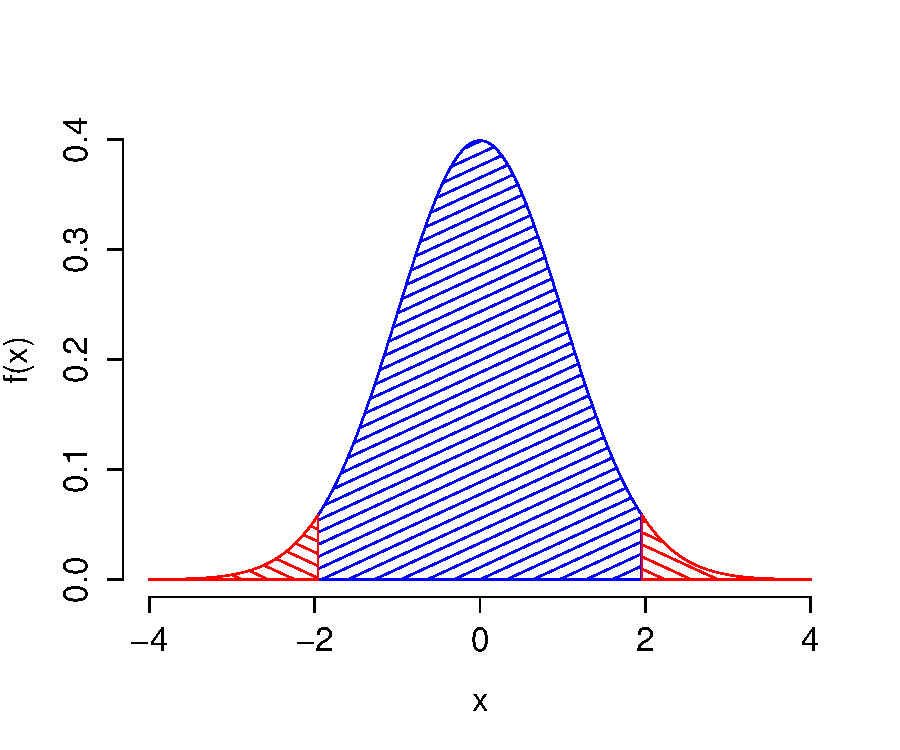
\includegraphics[scale = 0.6]{./images/normal_tails}
\end{figure}
\end{frame}
%%%%%%%%%%%%%%%%%%%%%%%%%%%%%%%%%%%%%%%%
\begin{frame}
\frametitle{Confidence Interval for a Normal Mean, $\sigma$ Known}
\Large
$$\boxed{\bar{X}_n \pm \texttt{qnorm}(1-\alpha/2) \times \sigma/\sqrt{n}}$$
\end{frame}
%%%%%%%%%%%%%%%%%%%%%%%%%%%%%%%%%%%%%%%%
\begin{frame}
\frametitle{What Affects the Margin of Error?}

	$$\boxed{\bar{X}_n \pm \texttt{qnorm}(1-\alpha/2) \times \sigma/\sqrt{n}}$$


	
\begin{block}{Sample Size $n$}
ME decreases with $n$: bigger sample $\implies$ tighter interval
\end{block}


\begin{block}{Population Std.\ Dev.\ $\sigma$}
ME increases with $\sigma$: more variable population $\implies$ wider interval
\end{block}



\begin{block}{Confidence Level $1-\alpha$}
ME increases with $1-\alpha$: higher conf.\ level $\implies$ wider interval

\pause

\vspace{1em}
	\begin{tabular}{r|lll}
	\hline
	Conf.\ Level & 90\% & 95\% & 99\% \\
	$\alpha$ & 0.1 & 0.05 & 0.01\\
	\texttt{qnorm}$(1-\alpha/2)$&1.64 & 1.96 & 2.56\\
	\hline
	\end{tabular}
\end{block}	
\end{frame}
%%%%%%%%%%%%%%%%%%%%%%%%%%%%%%%%%%%%%%%%

\begin{frame}
\frametitle{But What if $\sigma$ is Unknown?}
	\begin{itemize}
		\item What we've done so far assumed that $\sigma$ was known. 
		\item In real applications this is typically not the case. 
	\end{itemize}

\begin{alertblock}{Why not try using the sample standard deviation $s$?}
This works, but requires a small change. Instead of basing the interval on quantiles of a normal distribution, we need to use a $t$ distribution. We'll look at this next time.
\end{alertblock}

\end{frame}
%%%%%%%%%%%%%%%%%%%%%%%%%%%%%%%%%%%%%%%%




\end{document}